\providecommand{\destaque}[2]{{\setlength{\fboxsep}{1.5pt}\colorbox{#1}{$#2$}}}
\subsubsection{Interference and Covariance Matrix}\label{subsubsec:interferencia}

The interference from the non-target UEs reaches all $M$ antennas. Therefore, its covariance is an $M\times M$ matrix with non-zero off-diagonal entries. With $r$ non-target UEs, the received signal is:

\begin{equation}\label{eq:modelo-interferencia}
\mathbf y=
\mathbf H\mathbf s+\mathbf n=
\mathbf H\mathbf s+
\overline{\mathbf H}\,\overline{\mathbf s}
+\overline{\mathbf n},
\end{equation}

where $\overline{\mathbf H}\in\mathbb C^{M\times r}$ and $\overline{\mathbf s}\in\mathbb C^{r\times1}$ are the channels and the symbols of the non-target UEs, respectively, and $\overline{\mathbf n}$ is the thermal noise. The non-target UEs transmit with power $\beta$. Their signals are assumed to be independent of one another and of the thermal noise. Thus, the covariance matrix of the colored noise is \cite{zhao2025jsac,tomasin-interference}:
\begin{equation}\label{eq:Rn}
\mathbf R_n=
\beta\overline{\mathbf H}\,\overline{\mathbf H}^H
+\sigma^2\mathbf I_M
=
\begin{bmatrix}
r_{11} & \destaque{orange!40}{r_{12}} & \cdots & \destaque{orange!40}{r_{1M}}\\
\destaque{orange!40}{r_{21}} & r_{22} & \cdots & \destaque{orange!40}{r_{2M}}\\
\vdots & \vdots & \ddots & \vdots\\
\destaque{orange!40}{r_{M1}} & \destaque{orange!40}{r_{M2}} & \cdots & r_{MM}
\end{bmatrix}.
\end{equation}

The highlighted elements, outside the diagonal, come from the interference. Because of them, $\mathbf R_n$ is not block-diagonal, so it cannot be split into one independent block per cluster \cite{zhao2025jsac}.
% FONTE: zhao2025jsac paper.md:33, 105-113. Independência: hipótese do simulador.

Non-target UEs are usually located in neighboring cells. For simplicity, this work places the non-target UEs in the same cell as the target UEs and models them in the same way (Figure~\ref{fig:celula-interferencia}) \cite{zhao2025jsac}.
% FONTE: zhao2025jsac paper.md:33, 577.
\begin{figure}[!ht]
\caption{A cell with $K$ target UEs and $r$ non-target UEs. $\mathbf h_k$ and $\overline{\mathbf h}_r$ are the channels between a UE and the $M$ antennas of the BS.}
\label{fig:celula-interferencia}
\vspace{4pt}
\centering
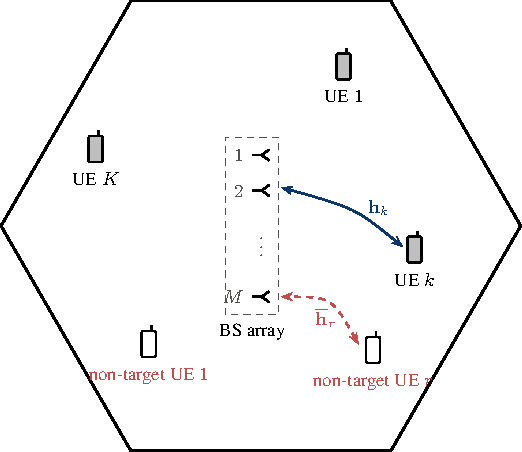
\includegraphics{Images/FLUXO/celula_interferencia.pdf}
\vspace{4pt}
\legend{Source: adapted from \citesp{marzetta2016fundamentals}, p.~32.}
\end{figure}
